\documentclass[11pt,a4paper]{article}

\usepackage[top=1.7cm,bottom=1.9cm,left=1.9cm,right=1.9cm]{geometry}
\usepackage{amsmath,amssymb}
\usepackage{booktabs}
\usepackage{graphicx}
\usepackage{caption}
\usepackage[hidelinks]{hyperref}
\usepackage{parskip}
\usepackage{titlesec}
\usepackage{float}

\titleformat{\section}{\normalfont\large\bfseries}{\thesection}{0.6em}{}
\titlespacing{\section}{0pt}{0.4em}{0.1em}

\setlength{\parskip}{2pt}
\setlength{\parindent}{0pt}

\title{\vspace{-2.5em}SF2943 Project --- Part B\\[1pt]
\large NVIDIA Daily Close Price Forecasting}
\author{Axel von Butovitsch, Brian Ooi, Eduardo Diogo Francisco Nazário, Joud Saardi, Tage Sköldefors}


\begin{document}
\maketitle
\vspace{-2em}

\section{Data}

We use daily closing prices of NVIDIA Corporation (NVDA) from Nasdaq Historical
Data, covering 2013-12-27 to 2026-04-17 ($n = 3093$ trading days, no missing values).
The raw series $X_t$ rose from \$0.39 to \$200.5 over this period, with variance
growing with the stock price increase (Figure~\ref{fig:raw}).

\section{Cleaning to Stationarity}

A log transform (Box--Cox $\lambda = 0$) stabilises the variance.
We then check for seasonality via harmonic regression.
A $k=1$ harmonic with period $d=252$ trading days captures a yearly cycle of
amplitude $\approx 0.110$ log units ($\approx 11\%$):
$
    \hat{s}_t^{(\text{year})} \;=\;
    +0.0660\cos\!\!\left(\tfrac{2\pi t}{252}\right)
    -0.0881\sin\!\!\left(\tfrac{2\pi t}{252}\right).
$
A $k=2$ harmonic with period $d=5$ (weekly) yielded amplitude $<0.003$ log units
and was dropped as negligible.
A polynomial trend was then fitted on the deseasonalised series. A quadratic was
selected by the thirds criterion but still left residuals with $\pm 1$ log unit
swings, indicating that a polynomial fit will not adequately captures NVIDIA's non-linear growth trajectory (flat 2013--2022, explosive 2023--2026). This was more or less expected as it is reasonable to assume that for NVIDIA's stock, the price is not correlated with any season-like behavior. We therefore apply first differencing to the log series, giving log returns $Y_t \;=\; \nabla\log X_t \;=\; \log X_t - \log X_{t-1}$ and remove any polynomial trend. This yields a visually
stationary series (Figure~\ref{fig:cleaning}).
The sample ACF of $Y_t$ has a single significant spike at lag~1
($\hat\rho(1) = -0.070$) and all other lags are within $\pm 1.96/\sqrt{n}$. 
Ljung--Box rejects iid ($Q(20)=52.8$, $p<0.001$), confirming residual structure
for the ARMA stage (Figure~\ref{fig:acf_pacf}).

\section{ARMA Fitting}

The single negative ACF/PACF spike at lag~1 motivates low-order candidates.
A grid search over ARMA$(p,q)$ with $p,q\leq 5$ by Gaussian MLE
and AICC nominally selects ARMA(5,4), but since there is ACF/PACF suggest that there is no evidence of lags beyond 1, we suspect that the improvement over simpler models is likely driven by volatility clustering rather than genuine autocorrelation.
Thus, we select \textbf{ARMA(2,0)} on grounds of parsimony (Table~\ref{tab:aicc}), with MLE estimates
$\hat\phi_1 = -0.068$ (se $= 0.013$),
$\hat\phi_2 = +0.032$ (se $= 0.014$),
$\hat\sigma^2 = 8.56\times10^{-4}$,
and constant $c = +0.002$ (average daily log return $\approx 0.2\%$).
All AR roots lie outside the unit disc, confirming causality.
Yule--Walker estimates agree with MLE to five decimal places, as expected.
Ljung--Box on the ARMA(2,0) residuals ($Q(20)=26.8$, df$=18$, $p=0.082$)
is consistent with white noise, so the model passes the residual whiteness test
(Figure~\ref{fig:arma_diag}).

\section{Forecasting}

Since $Y_t = \nabla\log X_t$, fitting ARMA(2,0) on log returns is equivalent to
ARIMA(2,1,0) on log prices.
The model is refit on the first $n-30$ observations and the $h$-step forecast
is computed via the innovations algorithm, then exponentiated
to recover price-level predictions with 95\% prediction intervals
(Figure~\ref{fig:forecast}).
We compare against a random walk with drift ARIMA(0,1,0) and a rolling
1-step-ahead forecast (model refit daily over the test window).
Results are given in Table~\ref{tab:forecast}.
ARIMA(2,1,0) and the random walk perform virtually identically
($\Delta\text{RMSE}<0.1$ USD), confirming the AR(2) correction adds
no meaningful predictive value at the 30-day horizon.
The rolling 1-step-ahead achieves RMSE $= 3.70$ USD, roughly three times lower,
reflecting daily price updating rather than model structure.

\section{Discussion}

The near-identical performance of ARIMA(2,1,0) and the random walk is consistent
with the efficient market hypothesis. Past returns contain almost no exploitable
information about future returns, and the model reduces to a drift plus a 2-day
AR correction that vanishes within 3 steps.
The main limitation is volatility clustering: variance is clearly non-constant
(Figure~\ref{fig:cleaning}), particularly around the 2020 COVID crash and 2022
sell-off, a feature better handled by GARCH-type models.
Quarterly earnings announcements (Feb, May, Aug, Nov) drive many of the large
spikes in $Y_t$; since their direction is unpredictable, they cannot be absorbed
by the ARMA conditional mean and represent an irreducible source of forecast error.

\section{Appendix}

\begin{figure}[H]
    \centering
    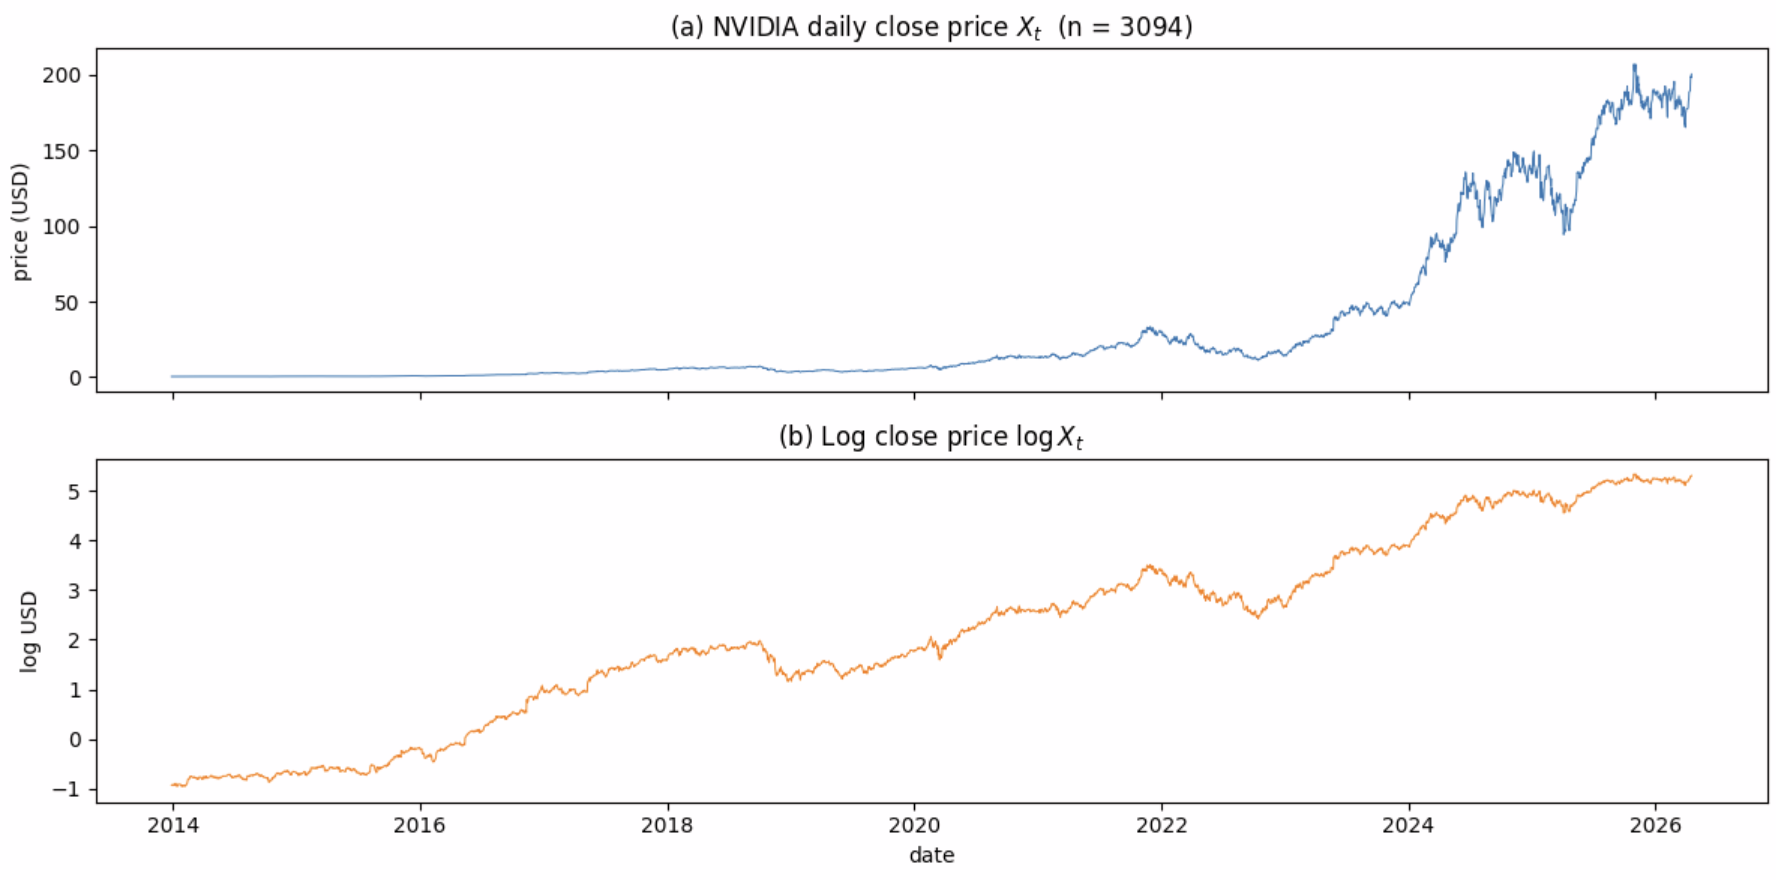
\includegraphics[width=0.88\linewidth]{raw_and_log.png}
    \caption{(a) Raw NVIDIA daily close price $X_t$ ($n = 3093$).
             (b) Log close price $\log X_t$ used for subsequent analysis.}
    \label{fig:raw}
\end{figure}

\begin{figure}[H]
    \centering
    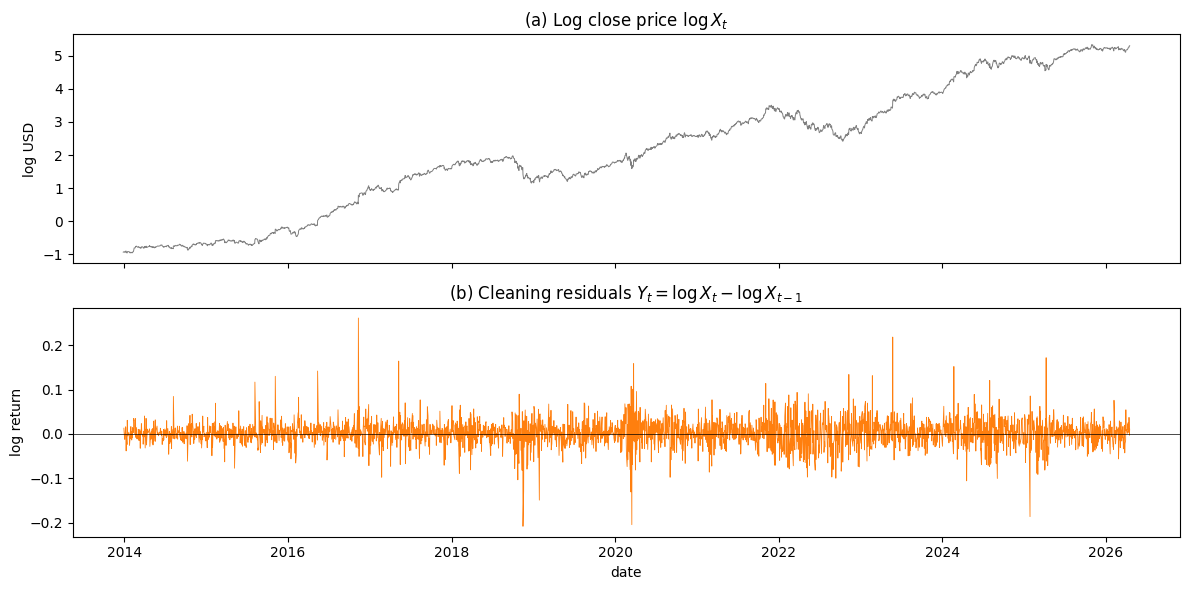
\includegraphics[width=0.88\linewidth]{cleaning_residuals.png}
    \caption{(a) Log close price $\log X_t$.
             (b) Cleaning residuals $Y_t = \log X_t - \log X_{t-1}$ (log returns).
             The series is stationary with isolated spikes around 2020 (COVID crash)
             and 2022 (rate hike sell-off).}
    \label{fig:cleaning}
\end{figure}


\begin{figure}[H]
    \centering
    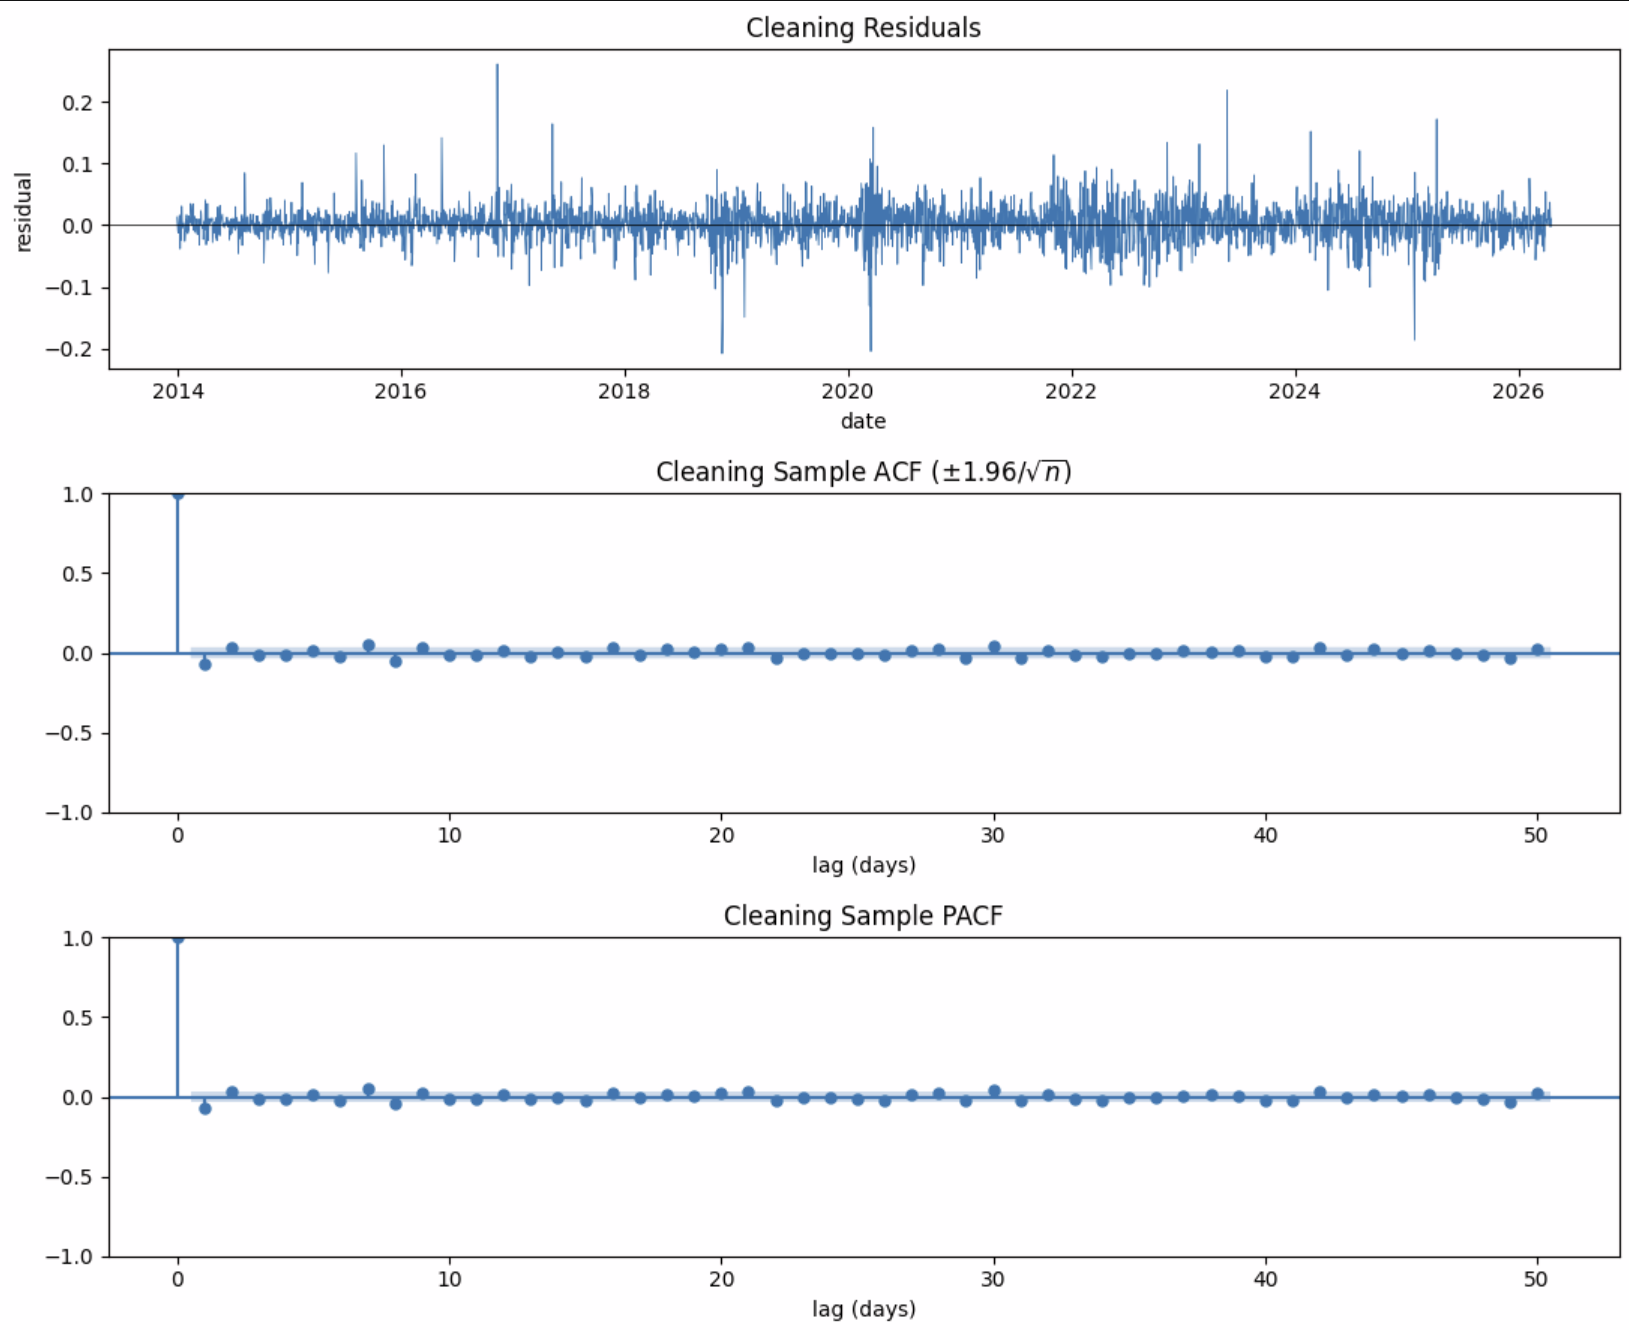
\includegraphics[width=0.88\linewidth]{acf_pacf_cleaning.png}
    \caption{Sample ACF and PACF of log returns $Y_t$ (lags 0--50,
             blue bands at $\pm 1.96/\sqrt{n}$).
             A single negative spike at lag 1 motivates low-order ARMA candidates.}
    \label{fig:acf_pacf}
\end{figure}

\begin{table}[H]
\centering
\caption{AICC values and causality/invertibility for candidate models.}
\label{tab:aicc}
\begin{tabular}{lrrrr}
\toprule
Model & $p+q$ & AICC & Causal & Invertible \\
\midrule
ARMA(2,0) & 2 & $-13059.67$ & Yes & Yes \\
ARMA(0,2) & 2 & $-13059.32$ & Yes & Yes \\
ARMA(1,1) & 2 & $-13058.92$ & Yes & Yes \\
\bottomrule
\end{tabular}
\end{table}

\begin{table}[H]
\centering
\caption{ARMA(2,0) Gaussian MLE estimates with standard errors.}
\label{tab:params}
\begin{tabular}{lrr}
\toprule
Parameter & Estimate & Std.\ Error \\
\midrule
$c$           & $+0.00201$ & $0.00052$ \\
$\hat\phi_1$  & $-0.06795$ & $0.01271$ \\
$\hat\phi_2$  & $+0.03187$ & $0.01448$ \\
$\hat\sigma^2$& $+0.000856$& $0.000011$ \\
\bottomrule
\end{tabular}
\end{table}


\begin{figure}[H]
    \centering
    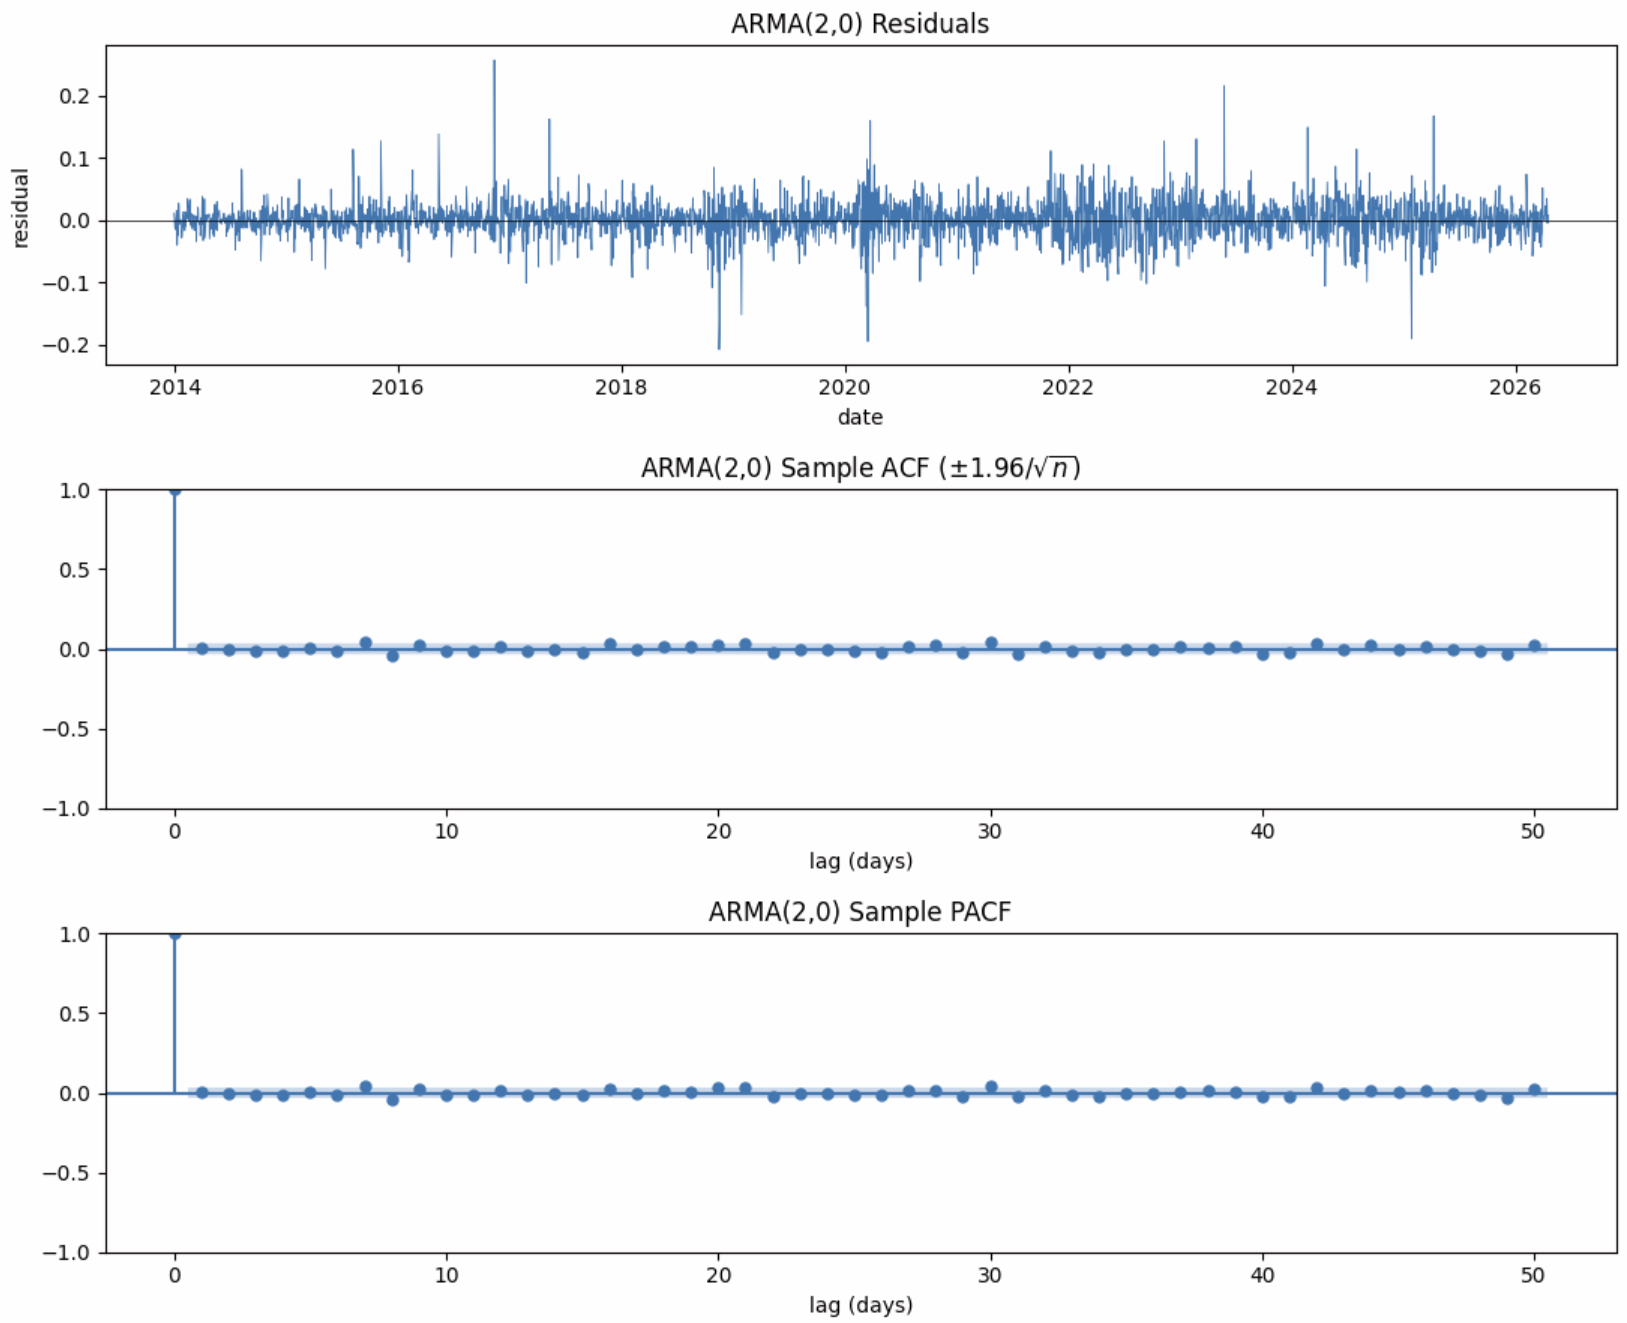
\includegraphics[width=0.88\linewidth]{arma_residuals.png}
    \caption{ARMA(2,0) residual diagnostics.
             ACF and PACF show no significant structure; Ljung--Box $p = 0.082$
             is consistent with white noise.}
    \label{fig:arma_diag}
\end{figure}

\begin{figure}[H]
    \centering
    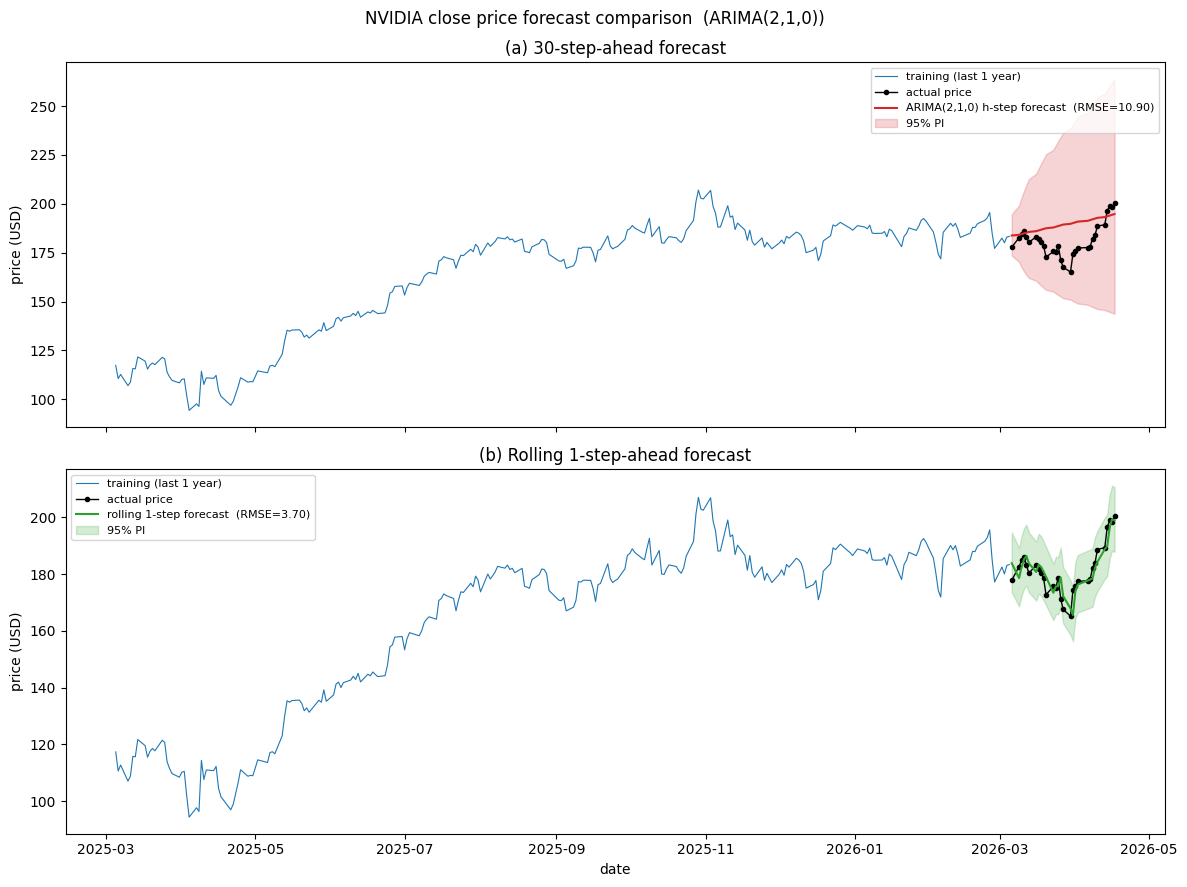
\includegraphics[width=0.88\linewidth]{forecast_comparison.png}
    \caption{(a) 30-step-ahead ARIMA(2,1,0) forecast with 95\% PI.
             (b) Rolling 1-step-ahead forecast with 95\% PI.
             Black markers: held-out actual prices.}
    \label{fig:forecast}
\end{figure}



\begin{table}[H]
\centering
\caption{Forecast evaluation on the 30-day out-of-time test set.}
\label{tab:forecast}
\begin{tabular}{lrrr}
\toprule
Model & RMSE (USD) & MAE (USD) & Coverage (95\%) \\
\midrule
ARIMA(2,1,0) --- $h$-step  & 10.90 & 8.94 & 1.00 \\
Random walk --- $h$-step   & 10.83 & 8.89 & 1.00 \\
ARIMA(2,1,0) --- rolling 1-step & 3.70 & 2.96 & 1.00 \\
\bottomrule
\end{tabular}
\end{table}



\end{document}